\chapter{Evitación de obstáculos}

La evitación de obstáculos desarrollada en este proyecto se apoya en el 
trabajo realizado previamente en el proyecto de investigación tutelado~\cite{estudio-nav2D}. En dicho 
estudio se analizó la viabilidad de implementar un sistema de evitación visual de obstáculos para drones de bajo 
coste empleando únicamente una cámara monocular RGB. Esta restricción imponía dos requisitos fundamentales: extraer información geométrica 
suficiente a partir de una única imagen y mantener una velocidad de procesamiento compatible con una aplicación en tiempo real.

El trabajo previo se centró principalmente en el estudio comparativo de distintos modelos de estimación 
de profundidad monocular y en la definición de una arquitectura de software capaz de ejecutarlos de forma 
eficiente. Para ello se evaluaron diferentes alternativas, entre ellas MiDaS~\cite{Ranftl2020}, Depth 
Anything~\cite{cheng2024depthanything} y otros modelos recientes de estimación de profundidad, valorando 
aspectos como la velocidad de inferencia, la estabilidad temporal, la precisión relativa de la 
profundidad y la posibilidad de integración en una arquitectura acelerada. Asimismo, se estudió 
el uso de modelos en formato ONNX~\cite{onnx_repo}, junto con técnicas de optimización basadas en 
ejecución multihilo y aceleración mediante GPU, con el objetivo de reducir la latencia total del 
sistema.

Aunque los resultados obtenidos demostraron la viabilidad general del enfoque, también pusieron de 
manifiesto algunas limitaciones importantes. La principal dificultad residía en que los estimadores de 
profundidad relativa no proporcionan directamente una distancia métrica absoluta, por lo que no siempre 
resulta trivial distinguir entre un obstáculo realmente peligroso y una variación de profundidad sin 
relevancia para la navegación.

El algoritmo desarrollado en este nuevo proyecto parte de esas conclusiones y propone una arquitectura 
de evitación más robusta. En lugar de basarse únicamente en el gradiente global del mapa de profundidad, 
se emplea un estimador más avanzado, \textit{Depth Anything 3}~\cite{overview-da}, y se añade una etapa 
específica de postprocesado orientada a la toma de decisiones. Esta etapa analiza la distribución de 
profundidad mediante segmentación y regiones de interés. De esta forma, el sistema no solo estima hacia 
dónde conviene desplazar la referencia lateral de evasión, sino que también determina si la situación requiere realmente una 
maniobra de evasión.

\section{Arquitectura}
\begin{figure}[H]
    \centering
    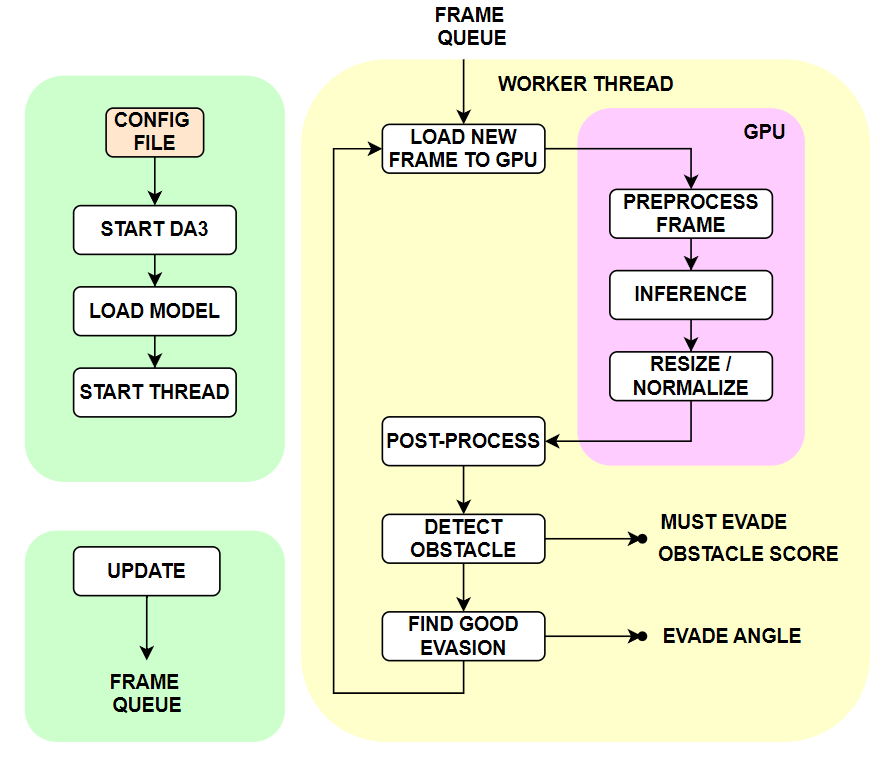
\includegraphics[width=1\textwidth]{images/depth_arq.png}
    \caption{Arquitectura del evitador de obstáculos. Fuente: Elaboración propia}
    \label{fig:evit_obs_arq}
\end{figure}

Como se observa en la Figura~\ref{fig:evit_obs_arq}, se propone una arquitectura acelerada por hardware, haciendo uso de 
la GPU y de CUDA tanto para ejecutar la inferencia del modelo como para realizar las operaciones de procesado mediante 
OpenCV~\cite{opencv_repo}.

En este módulo se distingue una primera etapa de inicialización, encargada de preparar el sistema, cargar el modelo 
utilizado y lanzar el hilo responsable de gestionar la comunicación con la GPU y calcular las diferentes métricas 
empleadas para la detección y evitación de obstáculos.

El funcionamiento general es sencillo: el hilo de trabajo (\textit{worker thread}) se encarga de realizar todo el proceso capturando 
siempre la imagen más reciente disponible en una cola interna. Dicha cola se actualiza cada vez que se recibe un nuevo 
\textit{fotograma} procedente de la cámara del UAV.

La salida principal del módulo se compone de tres parámetros:

\begin{enumerate}
    \item \texttt{evade\_angle} (\textit{float}): ángulo en 2D, expresado en coordenadas de imagen, que apunta hacia la 
    mejor dirección encontrada para evitar los obstáculos presentes en la escena.
    \item \texttt{obstacle\_score} (\textit{float}): indicador de riesgo asociado a la presencia de un obstáculo. Cuanto 
    mayor es su valor, mayor es la confianza del sistema en que existe un obstáculo cercano en la zona de avance.
    \item \texttt{must\_evade} (\textit{bool}): variable booleana encargada de indicar al planificador local cuándo debe 
    utilizar el ángulo de evasión y la puntuación de obstáculo calculados por el módulo.
\end{enumerate}

\section{Estimador de profundidad}
\subsection{Modelos y estudio de eficiencia}

Existen múltiples modelos de estimación de profundidad monocular, aunque no todos son adecuados para una arquitectura en 
tiempo real. Muchos de ellos presentan una elevada carga computacional. Por este motivo, en el proyecto 
previo~\cite{estudio-nav2D} se realizó un primer descarte de alternativas, atendiendo principalmente a la calidad de la 
profundidad estimada, la estabilidad visual entre fotogramas y la viabilidad de ejecución en tiempo real.

Tras dicho estudio inicial, las familias de modelos más prometedoras fueron MiDaS~\cite{Ranftl2020} y 
Depth Anything~\cite{cheng2024depthanything}. MiDaS destacaba por su robustez y por disponer de versiones relativamente 
ligeras, mientras que Depth Anything ofrecía una mejor generalización en escenas diversas y una estimación de profundidad 
visualmente más consistente. A partir de esta selección previa, en este proyecto se llevó a cabo un análisis más exhaustivo 
centrado en la eficiencia de inferencia, comparando distintos motores de ejecución, variantes de tamaño de los modelos y 
diferencias entre CPU y GPU.

El objetivo de esta comparación no era únicamente determinar qué modelo ofrecía mejores mapas de profundidad, sino 
seleccionar una configuración que permitiera integrar la estimación de profundidad dentro del sistema completo de 
evitación de obstáculos. Para ello se evaluaron principalmente dos motores de inferencia: OpenCV DNN~\cite{opencv_repo} y 
ONNX Runtime~\cite{onnx_repo}. Además, se comparó la ejecución sobre CPU y sobre GPU, ya que la arquitectura final del 
sistema debía aprovechar la aceleración por hardware disponible.

Las pruebas se realizaron sobre secuencias de 400 fotogramas, midiendo el tiempo medio, mínimo y la frecuencia de inferencia en fotogramas/s. La 
Tabla~\ref{tab:depth_models_efficiency} resume los resultados más relevantes obtenidos.

\begin{table}[H]
    \centering
    \caption{Comparación de eficiencia entre modelos y motores de inferencia.}
    \label{tab:depth_models_efficiency}
    \resizebox{\textwidth}{!}{
    \begin{tabular}{llcccc}
        \hline
        \textbf{Modelo} & \textbf{Motor} & \textbf{Dispositivo} & \textbf{Tiempo medio [ms]} & \textbf{Tiempo mín. [ms]} & \textbf{Fotogramas/s} \\
        \hline
        \texttt{model-small.onnx} & OpenCV & GPU & 13,337 & 10,876 & 74,98 \\
        \texttt{model-small.onnx} & ORT & GPU & 11,242 & 10,984 & 88,95 \\
        \texttt{model-small.onnx} & OpenCV & CPU & 85,849 & 67,114 & 11,65 \\
        \texttt{model-small.onnx} & ORT & CPU & 20,011 & 16,870 & 49,97 \\
        \hline
        \texttt{model-f6b98070.onnx} & OpenCV & GPU & 137,412 & 115,193 & 7,28 \\
        \texttt{model-f6b98070.onnx} & ORT & GPU & 112,439 & 96,194 & 8,89 \\
        \texttt{Depth-Anything-V2.onnx} & OpenCV & GPU & 116,233 & 109,870 & 8,60 \\
        \texttt{Depth-Anything-V2.onnx} & ORT & GPU & 116,149 & 101,537 & 8,61 \\
        \texttt{depth\_anything\_v2\_vits.onnx} & ORT & GPU & 95,016 & 86,731 & 10,52 \\
        \texttt{DA3METRIC-LARGE.onnx} & ORT & GPU & 303,545 & 215,126 & 3,29 \\
        \hline
        \texttt{DA3METRIC-SMALL.onnx} & ORT-DA3 & GPU & 56,765 & 43,850 & 17,62 \\
        \texttt{DA3METRIC-SMALL.onnx} & ORT-DA3 & GPU, sin vídeo & 51,283 & 42,439 & 19,50 \\
        \hline
    \end{tabular}
    }
\end{table}

Los resultados muestran varias conclusiones relevantes. En primer lugar, ONNX Runtime ofrece, en general, mejores tiempos de inferencia que OpenCV DNN para los modelos evaluados. Esta diferencia es especialmente visible en el modelo ligero \texttt{model-small.onnx}, donde ONNX Runtime alcanza 88,95 fotogramas/s en GPU frente a los 74,98 fotogramas/s obtenidos con OpenCV. En CPU, la diferencia también es significativa, pasando de 85,849 ms con OpenCV a 20,011 ms con ONNX Runtime.

En segundo lugar, se observa que los modelos de mayor tamaño, aunque pueden proporcionar estimaciones de profundidad más completas o detalladas, presentan tiempos de inferencia demasiado elevados para el sistema propuesto. Por ejemplo, \texttt{DA3METRIC-LARGE.onnx} alcanza únicamente 3,29 fotogramas/s, lo que lo hace inviable para una aplicación de evitación de obstáculos en tiempo real. De forma similar, algunas variantes de Depth Anything V2 se sitúan alrededor de 8--10 fotogramas/s, valores insuficientes si se considera que el módulo debe ejecutarse junto con el resto de procesos del sistema.

Finalmente, la variante seleccionada fue \texttt{DA3METRIC-SMALL.onnx}, ejecutada mediante ONNX Runtime sobre GPU. Esta configuración alcanza un tiempo medio de 56,765 ms por fotograma, equivalente a 17,62 fotogramas/s, y mejora hasta 51,283 ms, es decir, 19,50 fotogramas/s, cuando se elimina la carga adicional asociada a la visualización de vídeo. Aunque no es el modelo más rápido en términos absolutos, representa un compromiso adecuado entre calidad de la estimación de profundidad, estabilidad temporal y coste computacional, por lo que se adopta como base para el algoritmo de evitación desarrollado en este trabajo. En cualquier caso, el hecho de utilizar una variante denominada \texttt{METRIC} no implica por sí mismo que toda la lógica posterior opere directamente sobre distancias físicas absolutas ya calibradas, ya que en el algoritmo propuesto la decisión de evitación se apoya principalmente en comparaciones relativas, percentiles y medidas de cercanía normalizada.

\subsection{Kernel de preprocesado}

Además de la selección del modelo y del motor de inferencia, una parte importante de la optimización se encuentra en el preprocesado de la imagen de entrada. Antes de ejecutar el modelo, cada fotograma capturado por la cámara debe adaptarse al formato esperado por la red neuronal. Este proceso incluye el redimensionado de la imagen, la conversión de formato de color, el cambio de disposición de memoria y la normalización de los valores de intensidad.

En una implementación directa, estas operaciones podrían realizarse en CPU mediante OpenCV. Sin embargo, esto obliga a copiar datos entre CPU y GPU antes de cada inferencia, aumentando la latencia total del sistema. Para evitar este cuello de botella, en este proyecto se implementó un kernel CUDA específico encargado de realizar el preprocesado directamente en memoria de GPU.

El flujo de preprocesado aplicado es el siguiente. En primer lugar, la imagen se redimensiona al tamaño de entrada del modelo. Después, se convierte el formato de color de BGR a RGB, ya que OpenCV trabaja por defecto en BGR, mientras que el modelo espera los canales en orden RGB. Finalmente, el kernel CUDA transforma la imagen de tipo \texttt{uint8} en un tensor \texttt{float32}, normalizado y organizado en formato CHW.

La normalización aplicada a cada canal se define como:

\[
I_c'(x,y)=\frac{I_c(x,y)/255-\mu_c}{\sigma_c},
\]

donde \(I_c(x,y)\) es el valor original del píxel en el canal \(c\), \(\mu_c\) es la media del canal y \(\sigma_c\) su desviación típica. En este caso se utilizan los valores habituales de normalización empleados en modelos entrenados sobre ImageNet:

\[
\mu = [0.485,\;0.456,\;0.406],
\]

\[
\sigma = [0.229,\;0.224,\;0.225].
\]

El kernel implementado recibe una imagen RGB en formato intercalado, es decir, con disposición HWC, y genera directamente el tensor de entrada del modelo en formato CHW:

\[
\text{HWC} \rightarrow \text{CHW}.
\]

Esto significa que, para una imagen de tamaño \(H \times W\), los valores de salida se almacenan en tres planos consecutivos de memoria:

\[
R[H \times W], \quad G[H \times W], \quad B[H \times W].
\]

Cada hilo CUDA procesa un píxel de la imagen. Para cada posición \((x,y)\), el kernel lee los tres canales RGB, los convierte a coma flotante, aplica la normalización y escribe el resultado en la posición correspondiente del tensor de salida. La estructura de ejecución se organiza mediante bloques de \(16 \times 16\) hilos, cubriendo toda la imagen mediante una malla bidimensional.

Esta implementación presenta varias ventajas. En primer lugar, reduce el número de copias entre CPU y GPU dentro de la cadena de procesado, ya que la imagen permanece en memoria de GPU desde el preprocesado hasta la inferencia una vez disponible en dicho entorno de ejecución. En segundo lugar, fusiona en una única operación la conversión de tipo, la normalización y el cambio de disposición de memoria. En tercer lugar, permite ejecutar el preprocesado en el mismo \textit{stream} CUDA que el resto de operaciones, facilitando una integración más eficiente con OpenCV CUDA y ONNX Runtime.

Por tanto, el kernel de preprocesado contribuye a reducir la latencia global del sistema y a mantener una arquitectura coherente con el objetivo de ejecución en tiempo real. En lugar de tratar la inferencia como una operación aislada, se optimiza toda la cadena de procesamiento: captura, transferencia a GPU, preprocesado, inferencia y postprocesado.

\section{Detección de obstáculos y cálculo de la dirección de evitación}
El módulo de evitación se basa en la salida de un estimador monocular de profundidad DA3. A partir de cada 
imagen RGB se obtiene un mapa de profundidad denso, sobre el que se calcula una señal de 
\textbf{activación de la evitación} y, una \textbf{dirección angular de escape}.

\subsection{Estimación de profundidad}
Sea \(I\) la imagen RGB. Esta imagen se redimensiona al tamaño de entrada de la red y se normaliza 
antes de ser inferida mediante el modelo DA3. La salida es un mapa de profundidad
\[D(x,y),\]
donde valores mayores representan regiones más lejanas y valores menores regiones más cercanas. En la práctica, para el algoritmo desarrollado en este trabajo, este mapa no se emplea directamente como una medida métrica absoluta robusta en metros para toda la lógica de decisión. En su lugar, se utiliza principalmente como una señal de ordenación espacial a partir de la cual se construyen medidas relativas de cercanía y espacio libre.

\subsection{Normalización de la profundidad}
Para eliminar posibles errores de cómputo se escogen los píxeles con valores dentro de un rango configurable \([d_{\min}, d_{\max}]\). En este contexto, dichos límites se utilizan como filtro práctico sobre la salida del modelo y no como una garantía de exactitud métrica absoluta en todo el rango. Denotando por \(D\) al mapa de profundidad bruto y por \(D_v\) al conjunto de profundidades válidas dentro de ese rango, primero se calcula la proporción de píxeles válidos y, a continuación, los percentiles \(p_{10}\) y \(p_{90}\) de \(D_v\). Con ellos se obtiene el mapa de profundidad normalizada:
\[
D_n(x,y) = \mathrm{clamp}\!\left(\frac{D(x,y) - p_{10}}{p_{90} - p_{10}},\, 0,\, 1\right).
\]

A continuación se define un mapa de cercanía:
\[C(x,y) = 1 - D_n(x,y).\]
De tal modo que \(C\approx 1\) indica proximidad o cercanía y \(C\approx 0\) lejanía. Por tanto, a partir de este punto la mayor parte de las decisiones del módulo se formulan en términos de cercanía normalizada y ocupación relativa, en lugar de depender exclusivamente de la magnitud absoluta de \(D\).

\subsection{Regiones de interés}
Uno de los principales problemas en el algoritmo primigenio era el uso de toda la imagen para el cálculo del gradiente, esto 
es un error ya que pueden existir casos donde el algoritmo no funcione, un ejemplo de ello puede ser un fotograma con una columna central lo 
suficientemente centrada como para que el gradiente salga 0, otro caso problemático es el caso donde existe demasiado obstáculo y por tanto 
la magnitud del vector de movimiento es demasiado baja. Es por ello que en el nuevo algoritmo se introduce el uso de regiones de interés:

\begin{itemize}
\item una \textbf{ROI frontal}, usada para decidir si existe un obstáculo peligroso delante del vehículo;
\item una \textbf{ROI de guiado}, usada para calcular hacia dónde conviene desplazarse.
\end{itemize}

Como se puede observar en la Figura~\ref{fig:roi_ex}, la ROI frontal concentra la detección en la zona relevante para la 
colisión, mientras que la ROI de guiado analiza un área más ancha para identificar una dirección lateral más despejada 
según los indicadores de cercanía y ocupación definidos.
\begin{figure}[H]
    \centering
    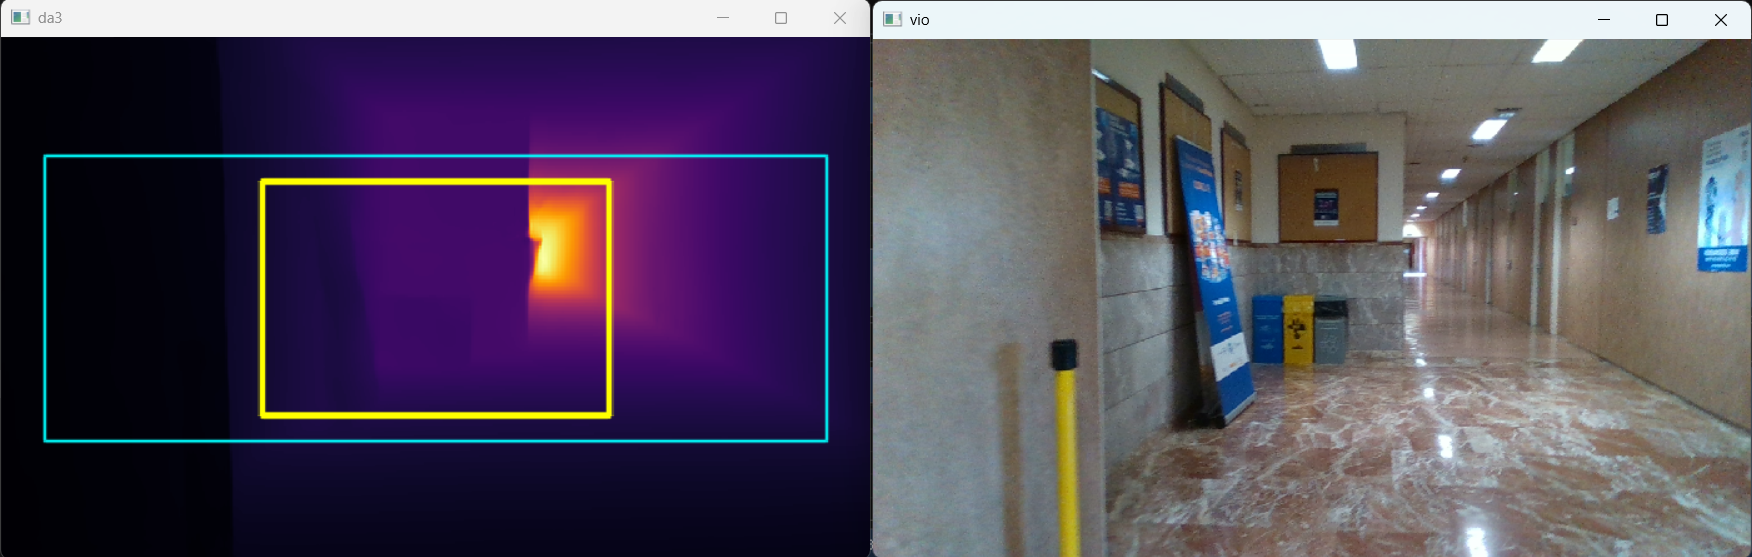
\includegraphics[width=1\textwidth]{images/roi_examp.png}
    \caption{ROI frontal en amarillo y ROI de guiado en azul. Fuente: Elaboración propia}
    \label{fig:roi_ex}
\end{figure}

\subsection{Máscara de ocupación frontal}
Dentro de la ROI frontal se umbraliza el mapa de cercanía para obtener una máscara binaria de obstáculo (\(M_F\)),~Figura \ref{fig:mask_obj}, obteniendo 1 en el caso 
de que el valor del píxel en \(C(ROI_F)\) sea mayor a un umbral de cercanía y 0 en otro caso. A partir de esta 
máscara y de la profundidad frontal se calculan las siguientes métricas:


\begin{figure}[H]
    \centering
    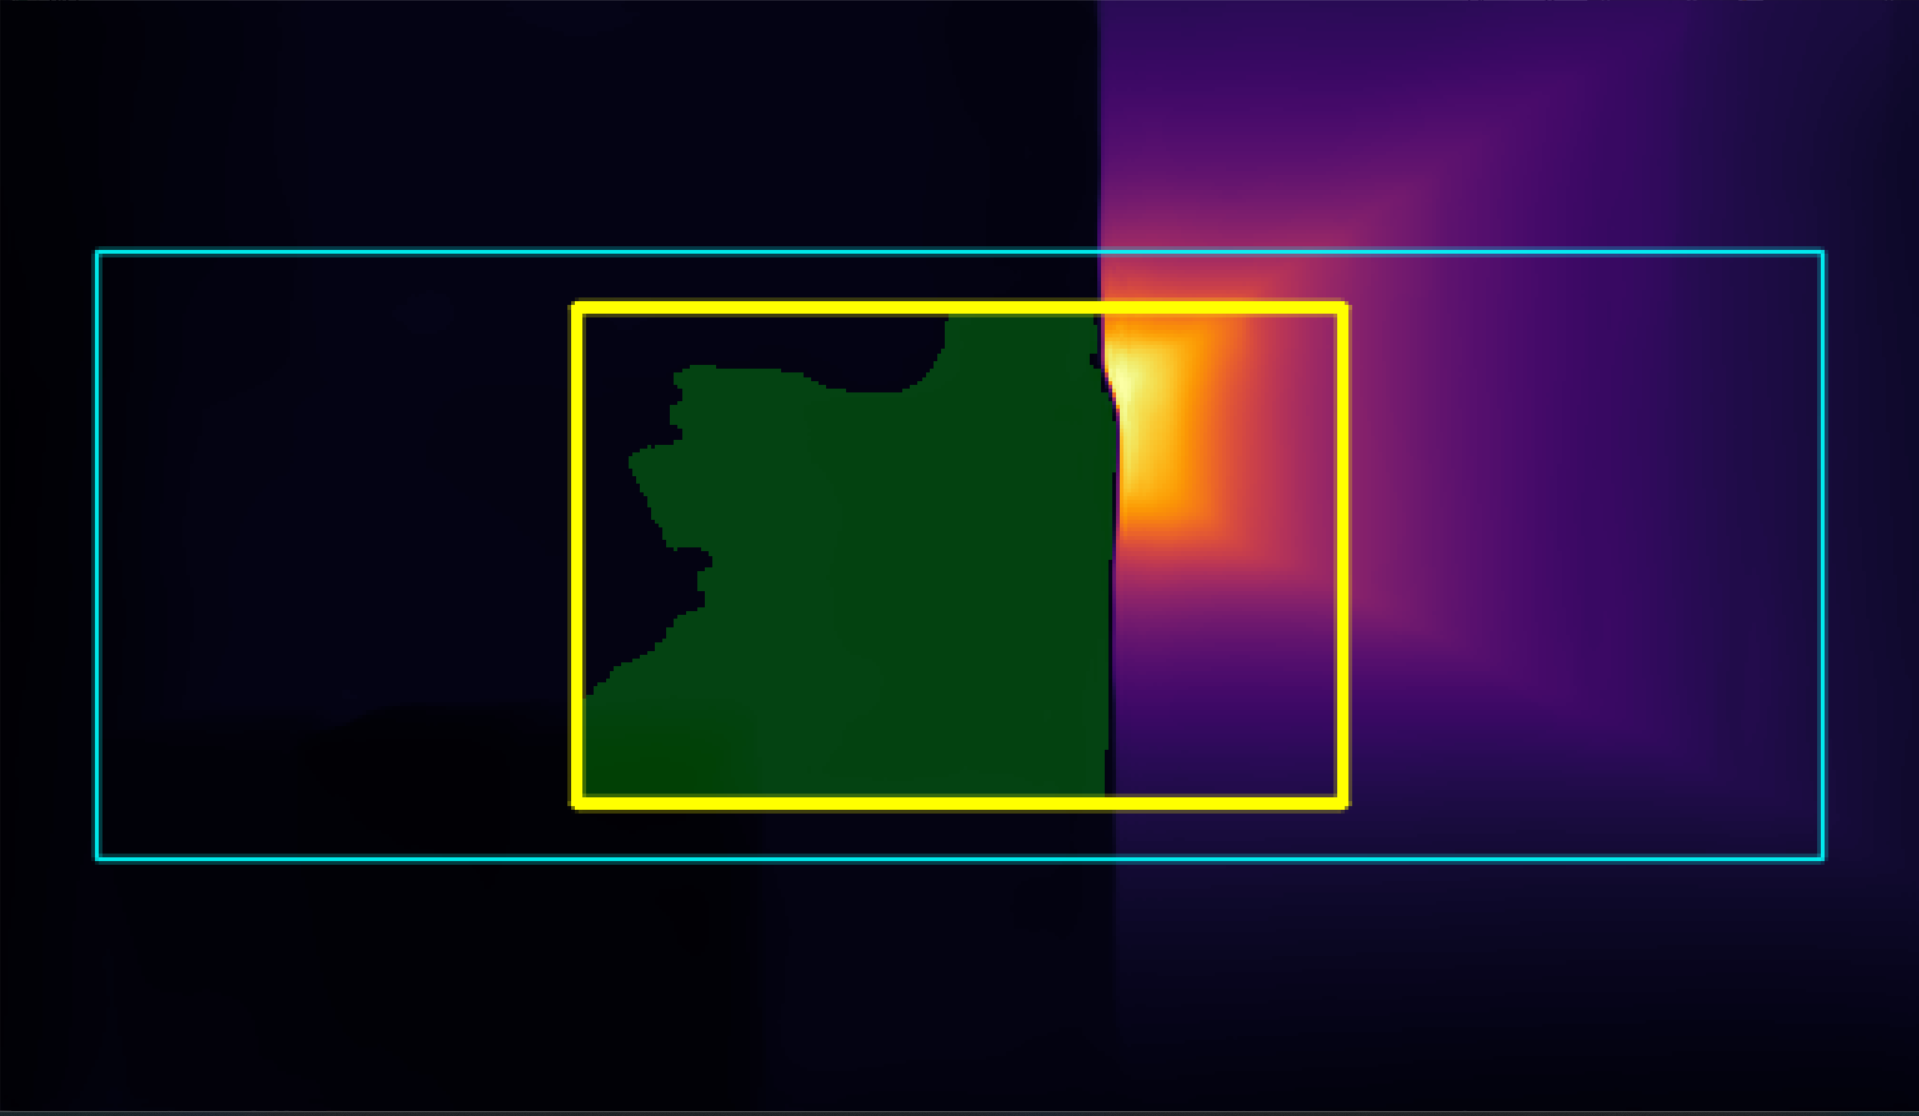
\includegraphics[width=1\textwidth]{images/mask_obj.png}
    \caption{Máscara \(M_F\) de la ROI frontal en verde. Fuente: Elaboración propia}
    \label{fig:mask_obj}
\end{figure}

\begin{itemize}
\item \textbf{Cercanía media frontal:} \(\bar{C}_F = \frac{1}{N_F}\sum C(ROI_F)\)

\item \textbf{Área ocupada:} \(A_F = \frac{1}{N_F}\sum M_F(ROI_F)\)

\item \textbf{Ratio de mayor área conexa:}\(B_F = \frac{\text{Mayor área conexa en } M_F}{N_F}\)

\item \textbf{Profundidad frontal percentil 20:} \(d_{20} = P_{20}(D_v \text{ en } ROI_F),\)

\item \textbf{Profundidad frontal pico:} \(d_{p} = P_{q}(D_v \text{ en } ROI_F)\)
donde \(q\) es un percentil pequeño, típicamente \(q=5\), para detectar obstáculos pequeños pero muy cercanos.
\end{itemize}

Estas dos últimas profundidades se convierten también a cercanía normalizada:

\[
c_{20} = \mathrm{clip}\!\left(1-\frac{d_{20}-p_{10}}{p_{90}-p_{10}},\,0,\,1\right),
\qquad
c_{p} = \mathrm{clip}\!\left(1-\frac{d_{p}-p_{10}}{p_{90}-p_{10}},\,0,\,1\right).
\]


\subsection{Cálculo de la puntuación de obstáculo}

Con las métricas anteriores se construye una puntuación escalar de obstáculo, esto se puede observar en la Figuras~\ref{fig:prop_noevad} y \ref{fig:prop_evad}:
\[ S_t = w_1 \bar{C}_F + w_2 A_F + w_3 B_F + w_4 c_{20} + w_5 c_p. \]


Esta puntuación se filtra temporalmente mediante un suavizado exponencial:

\begin{figure}[H]
    \centering
    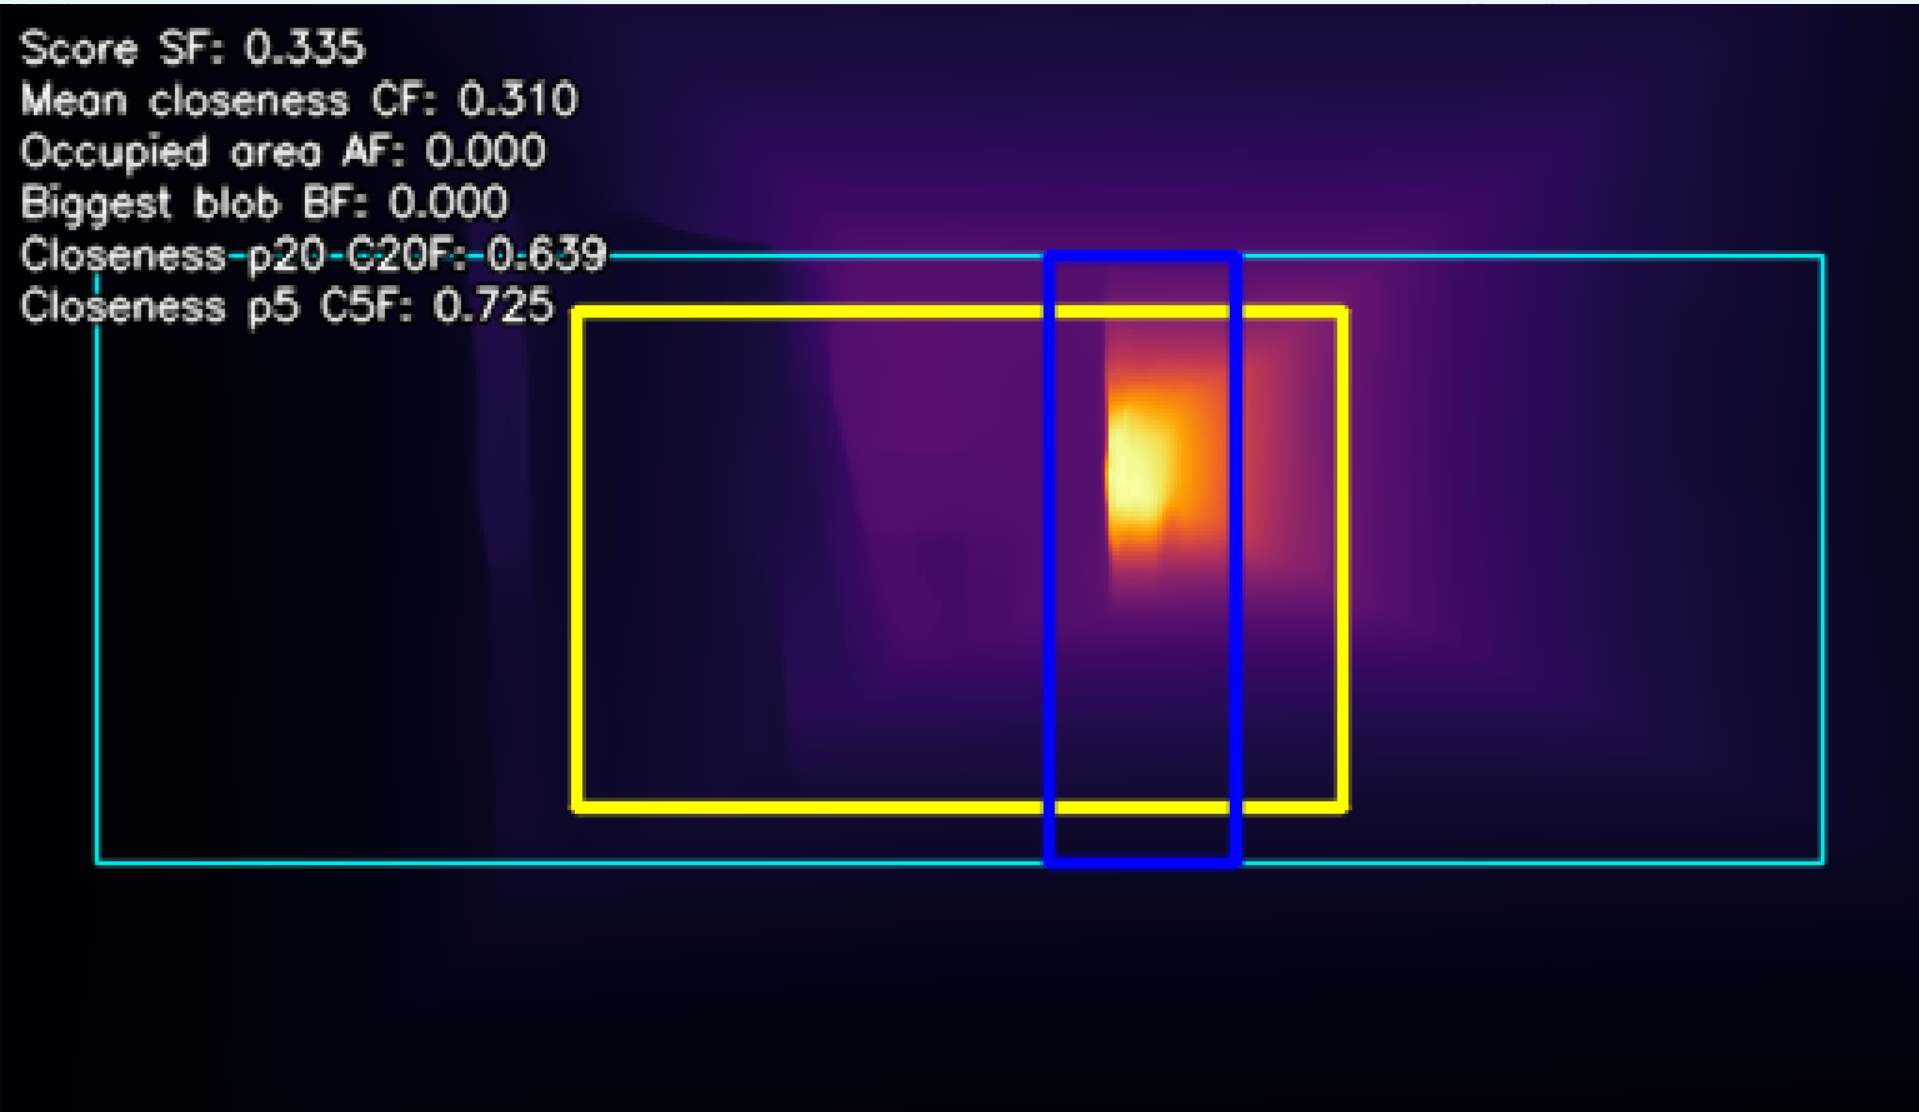
\includegraphics[width=1\textwidth]{images/prop_noevad.png}
    \caption{Ejemplo de propiedades sin obstáculo presente. Fuente: Elaboración propia}
    \label{fig:prop_noevad}
\end{figure}

\begin{figure}[H]
    \centering
    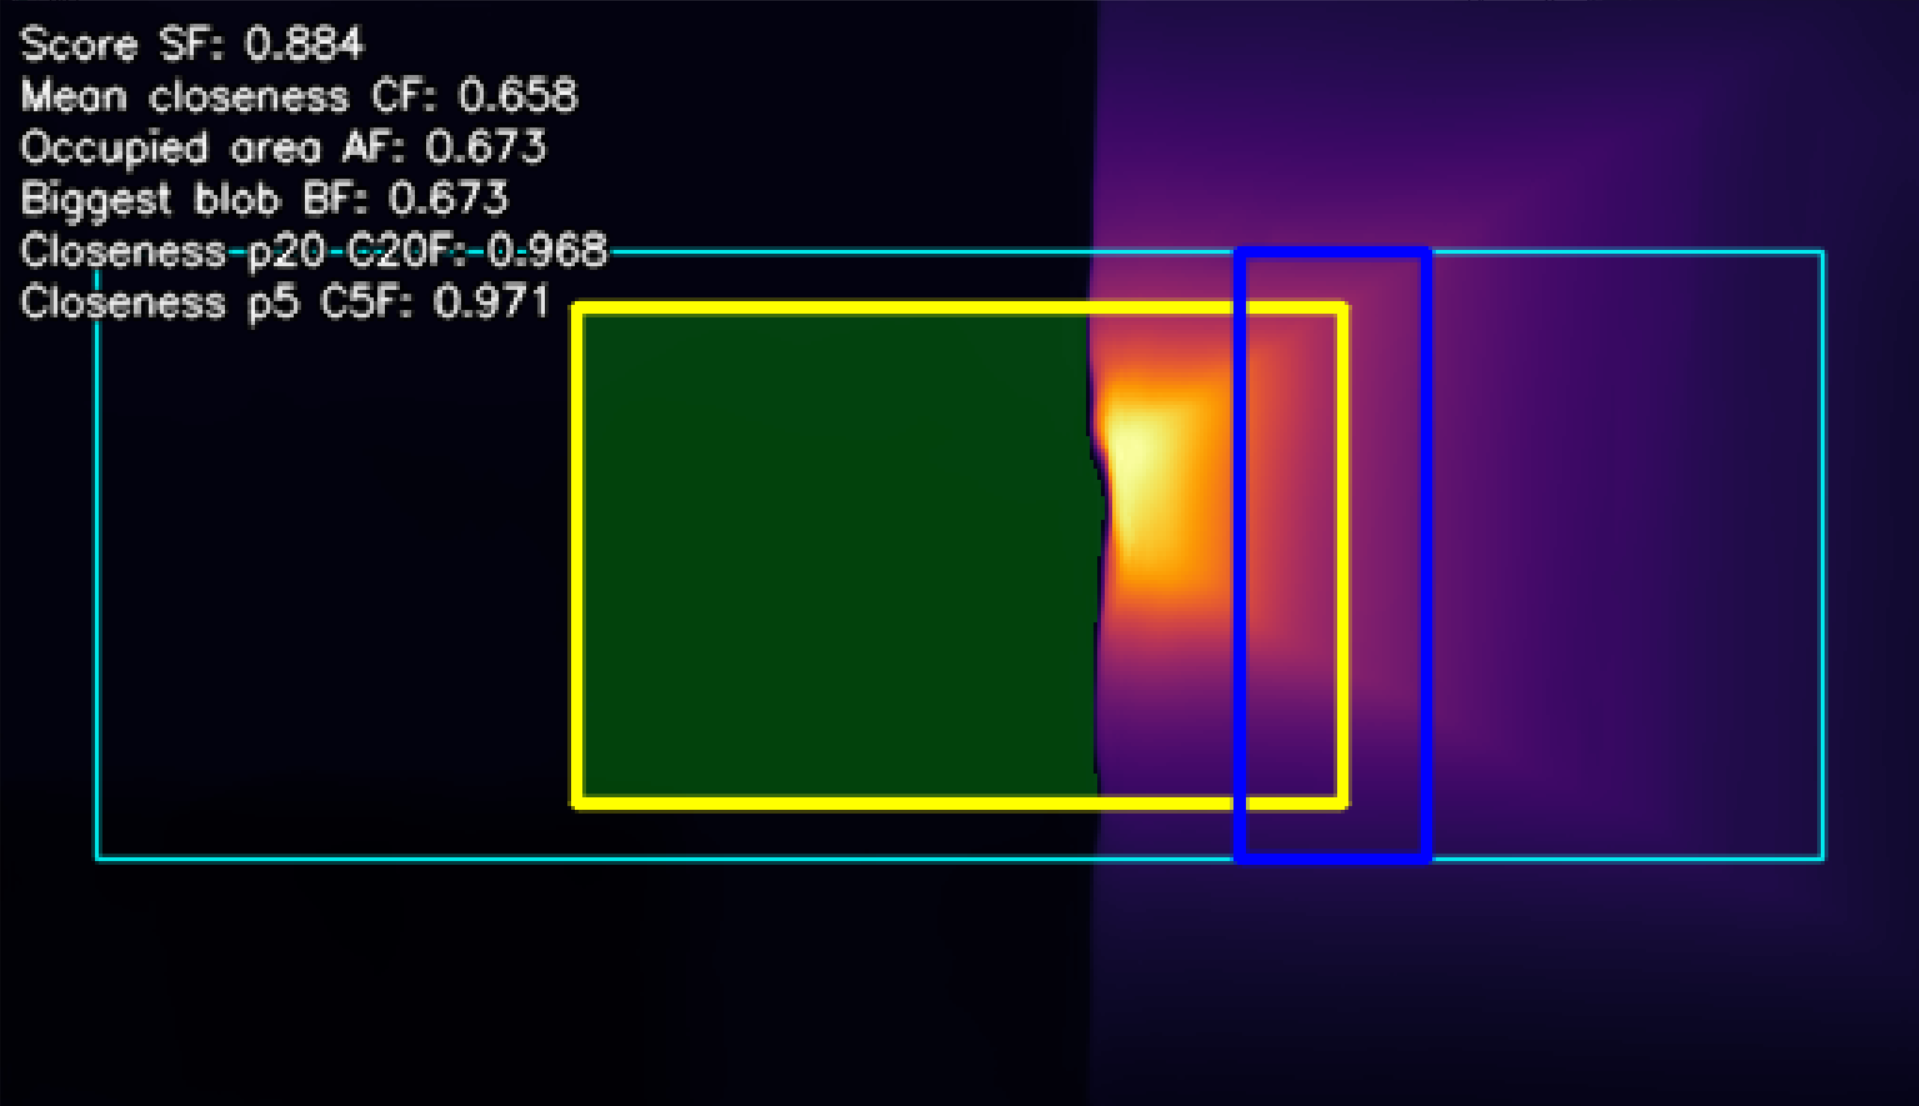
\includegraphics[width=1\textwidth]{images/prop_evad.png}
    \caption{Ejemplo de propiedades con obstáculo presente. Fuente: Elaboración propia}
    \label{fig:prop_evad}
\end{figure}


\[
\tilde{S}_t = \alpha_S \tilde{S}_{t-1} + (1-\alpha_S)S_t
\]
donde \(\alpha_S \in [0,1]\) es el factor de suavizado de la puntuación y \(\tilde{S}_t\) representa la puntuación filtrada.

\subsection{Activación del aviso de evitación}

La bandera binaria de evitación \(must\_evade\) indica si el módulo considera necesario avisar al planificador local de la 
presencia de un obstáculo frontal. Esta variable no se obtiene directamente del modelo de profundidad, sino a partir 
de una combinación de condiciones sobre la profundidad estimada, la ocupación de la región frontal y la puntuación global 
de obstáculo.

Para ello se definen varios umbrales:
\begin{itemize}
    \item El umbral \(d_{\text{evade}}\) representa un umbral operativo aplicado sobre la profundidad frontal estimada por el modelo para decidir si un obstáculo se considera relevante para la evasión. Aunque su valor se expresa en las mismas unidades manejadas por la salida del modelo, en este trabajo su uso debe interpretarse como un criterio práctico de activación dentro de la cadena completa de decisión, no como una medida física absoluta suficiente por sí sola. 
    \item El umbral \(T_p\) define el valor mínimo de cercanía pico (percentil 5\%) necesario para considerar que existe 
    una zona especialmente próxima al vehículo. 
    \item Los umbrales \(A_{\min}\) y \(B_{\min}\) establecen, respectivamente, el porcentaje mínimo de área cercana y el 
    tamaño mínimo del mayor obstáculo conexo dentro de la región frontal. 
    \item El umbral \(T_{\text{on}}\) es el umbral de activación de la puntuación global de obstáculo.
    \item El umbral \(T_{\text{off}}\) es el umbral de desactivación empleado para introducir histéresis.
\end{itemize}
Las condiciones de activación son las siguientes:

\begin{itemize}
    \item activación por profundidad frontal, cuando el percentil 20 de profundidad en la región frontal es menor o igual que el umbral operativo de evasión:
    \[d_{20} \le d_{\text{evade}}\]

    \item activación por cercanía pico, cuando la zona más próxima de la región frontal supera el umbral de cercanía definido:
    \[c_p \ge T_p\]

    \item activación por ocupación, cuando el área cercana o el mayor obstáculo conexo dentro de la región frontal superan sus respectivos umbrales:
    \[A_F \ge A_{\min} \quad \text{o} \quad B_F \ge B_{\min}\]

    \item activación por puntuación global, cuando la puntuación de obstáculo filtrada supera el umbral de activación:
    \[\tilde{S}_t \ge T_{\text{on}}\]
\end{itemize}

Estas condiciones se combinan en una única señal lógica de activación, denotada por \(\mathrm{threshold\_hit}_t\), de manera que sea suficiente el cumplimiento de una de ellas
para la activación de la bandera booleana:

\[
\mathrm{threshold\_hit}_t =
(d_{20} \le d_{\text{evade}}) || (c_p \ge T_p) || (A_F \ge A_{\min}) || (B_F \ge B_{\min}) || (\tilde{S}_t \ge T_{\text{on}}). \]

Una vez activado el aviso de evitación, la desactivación no se realiza con el mismo umbral de activación, sino con un umbral inferior \(T_{\text{off}}\). De este modo, si el sistema ya estaba en estado de evasión, la bandera se mantiene activa mientras la puntuación de obstáculo siga siendo suficientemente alta:

\[
\tilde{S}_t \ge T_{\text{off}}.
\]

Por tanto, la actualización final de la bandera de evitación queda definida como:

\[
\mathrm{must\_evade}_t =
\begin{cases}
1, & \text{si } \mathrm{must\_evade}_{t-1}=0 \text{ y } \mathrm{threshold\_hit}_t,\\
1, & \text{si } \mathrm{must\_evade}_{t-1}=1 \text{ y } \tilde{S}_t \ge T_{\text{off}},\\
0, & \text{en otro caso.}
\end{cases}
\]

Este comportamiento introduce una histéresis en la activación del aviso. El sistema se activa cuando 
alguna condición supera su umbral correspondiente, pero solo se desactiva cuando la puntuación global cae por debajo de 
\(T_{\text{off}}\). Al ser \(T_{\text{off}}\) menor que \(T_{\text{on}}\), se evita que la bandera \(must\_evade\) conmute 
rápidamente entre activa e inactiva cuando la escena se encuentra cerca del límite de decisión. Todo este comportamiento 
se puede comprobar en las Figuras~\ref{fig:mustevade_false} y \ref{fig:mustevade_true}.



\begin{figure}[H]
    \centering
    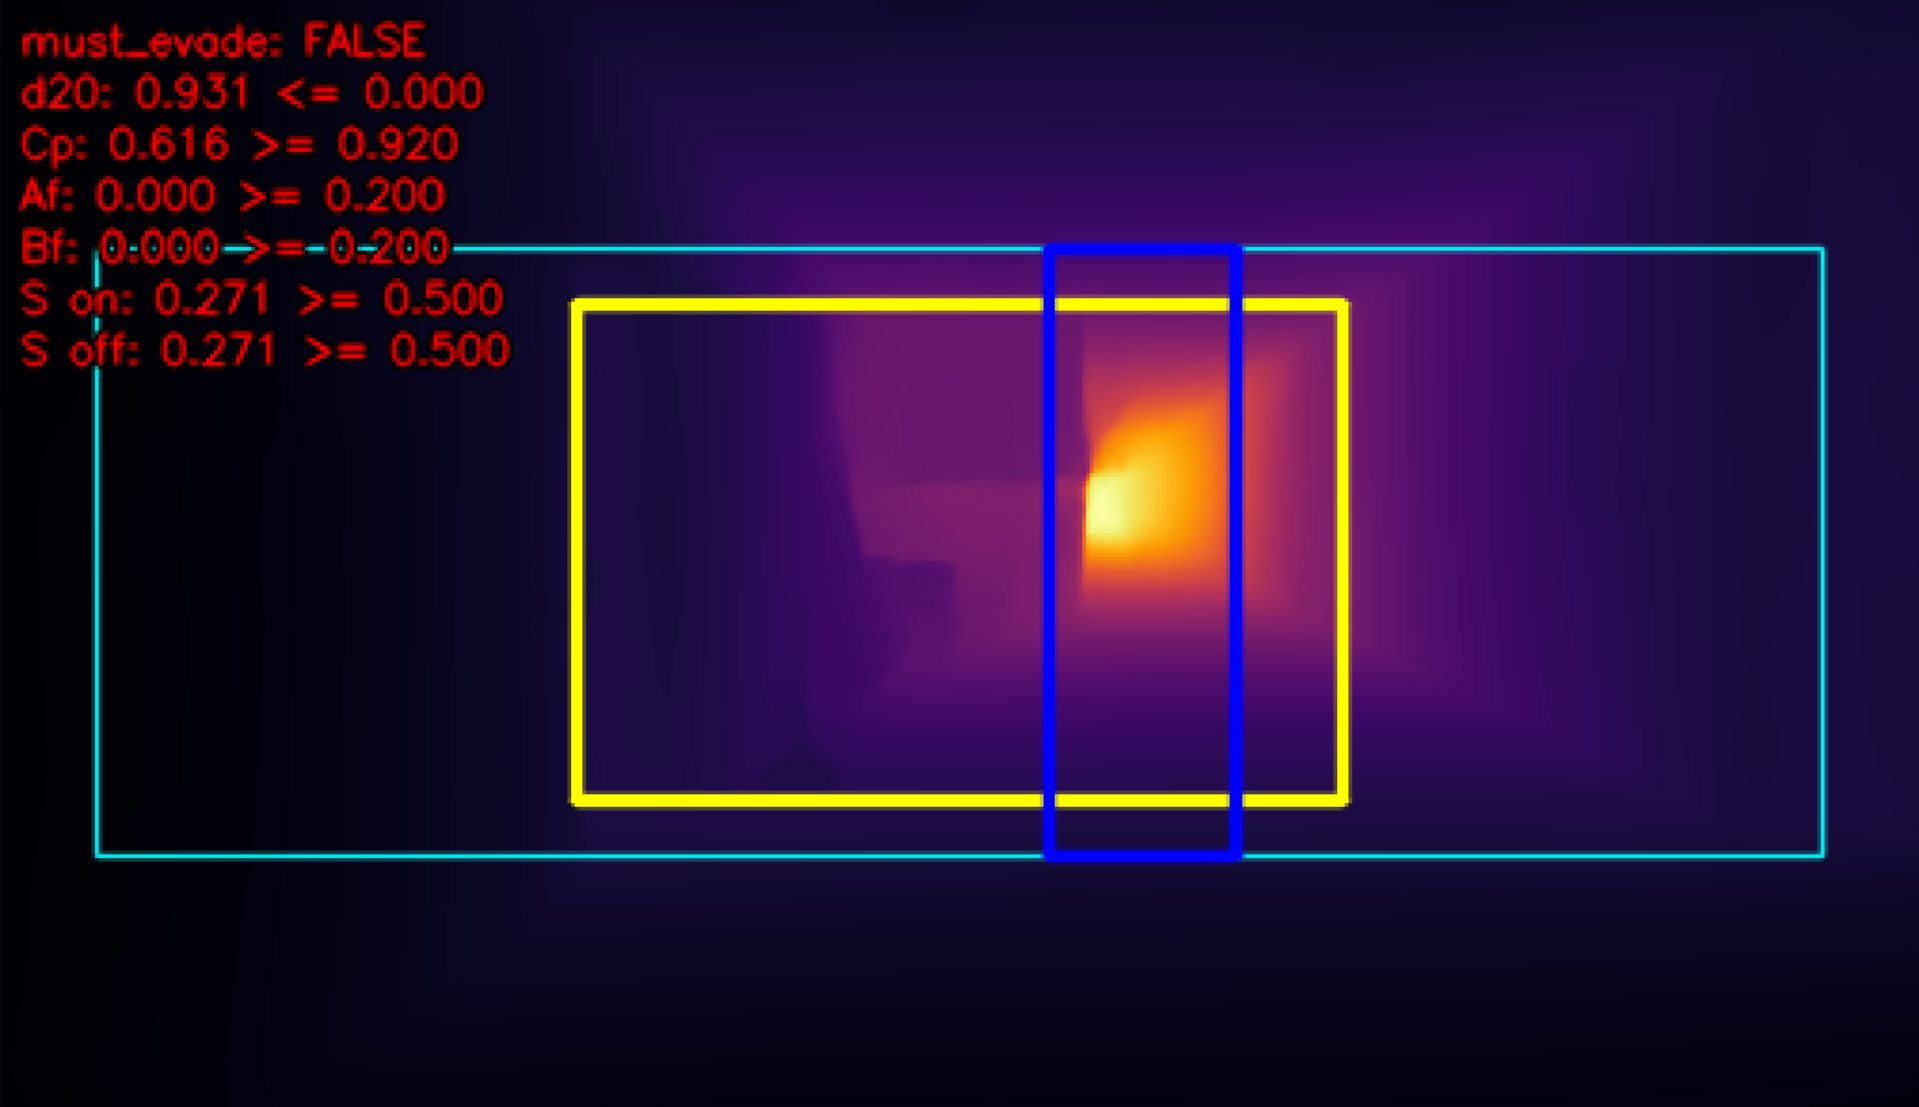
\includegraphics[width=1\textwidth]{images/mustevade_false.png}
    \caption{Ejemplo de condiciones no cumplidas. Fuente: Elaboración propia}
    \label{fig:mustevade_false}
\end{figure}

\begin{figure}[H]
    \centering
    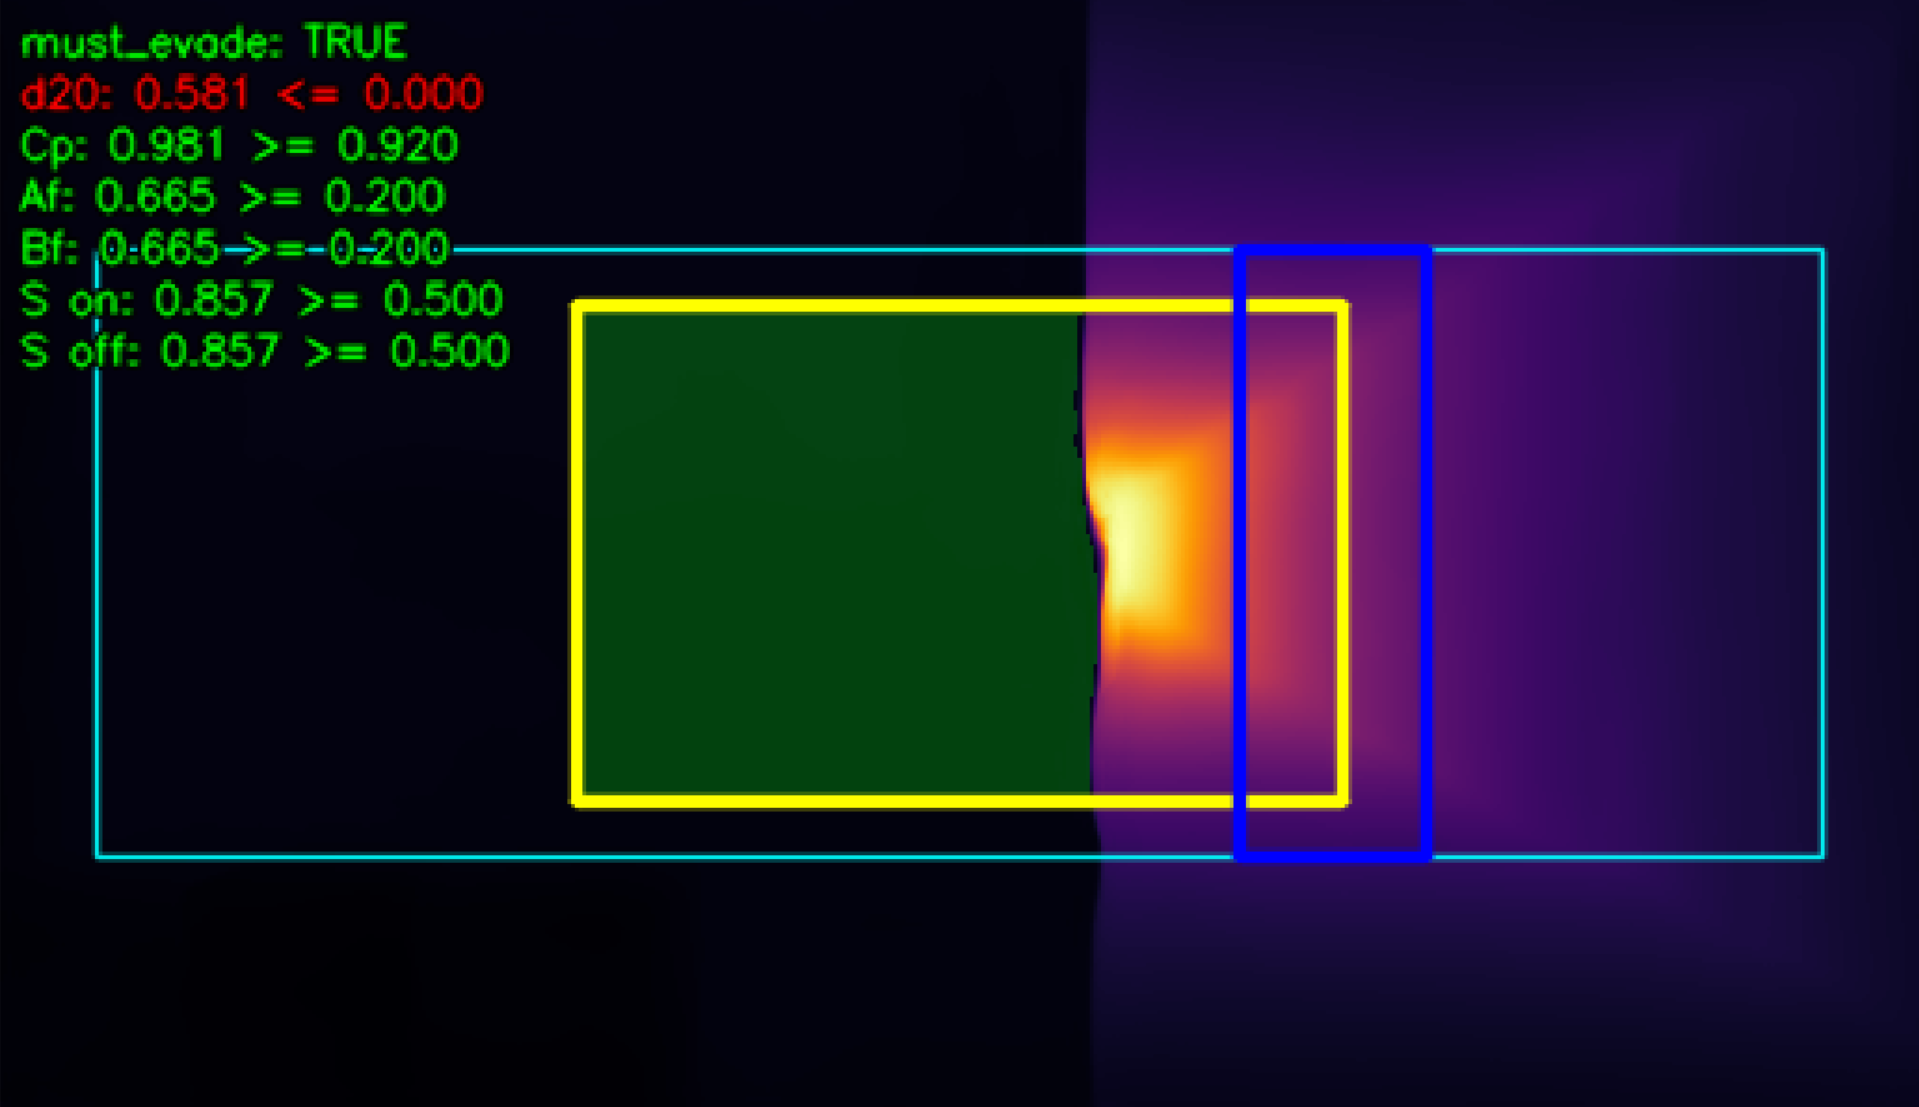
\includegraphics[width=1\textwidth]{images/mustevade_true.png}
    \caption{Ejemplo de condiciones cumplidas. Fuente: Elaboración propia}
    \label{fig:mustevade_true}
\end{figure}


\subsection{Cálculo de la dirección de evitación}

La dirección de evitación se calcula identificando hacia qué zona de la imagen conviene desplazar la referencia lateral 
de evasión. Para ello, se utiliza la ROI de guiado, que corresponde a una región amplia de la imagen centrada en la zona 
de avance del UAV. Esta región se divide en varios sectores verticales, de forma que cada uno de ellos representa una 
posible dirección lateral de escape como se puede ver en la Figura~\ref{fig:sectors}.


\begin{figure}[H]
    \centering
    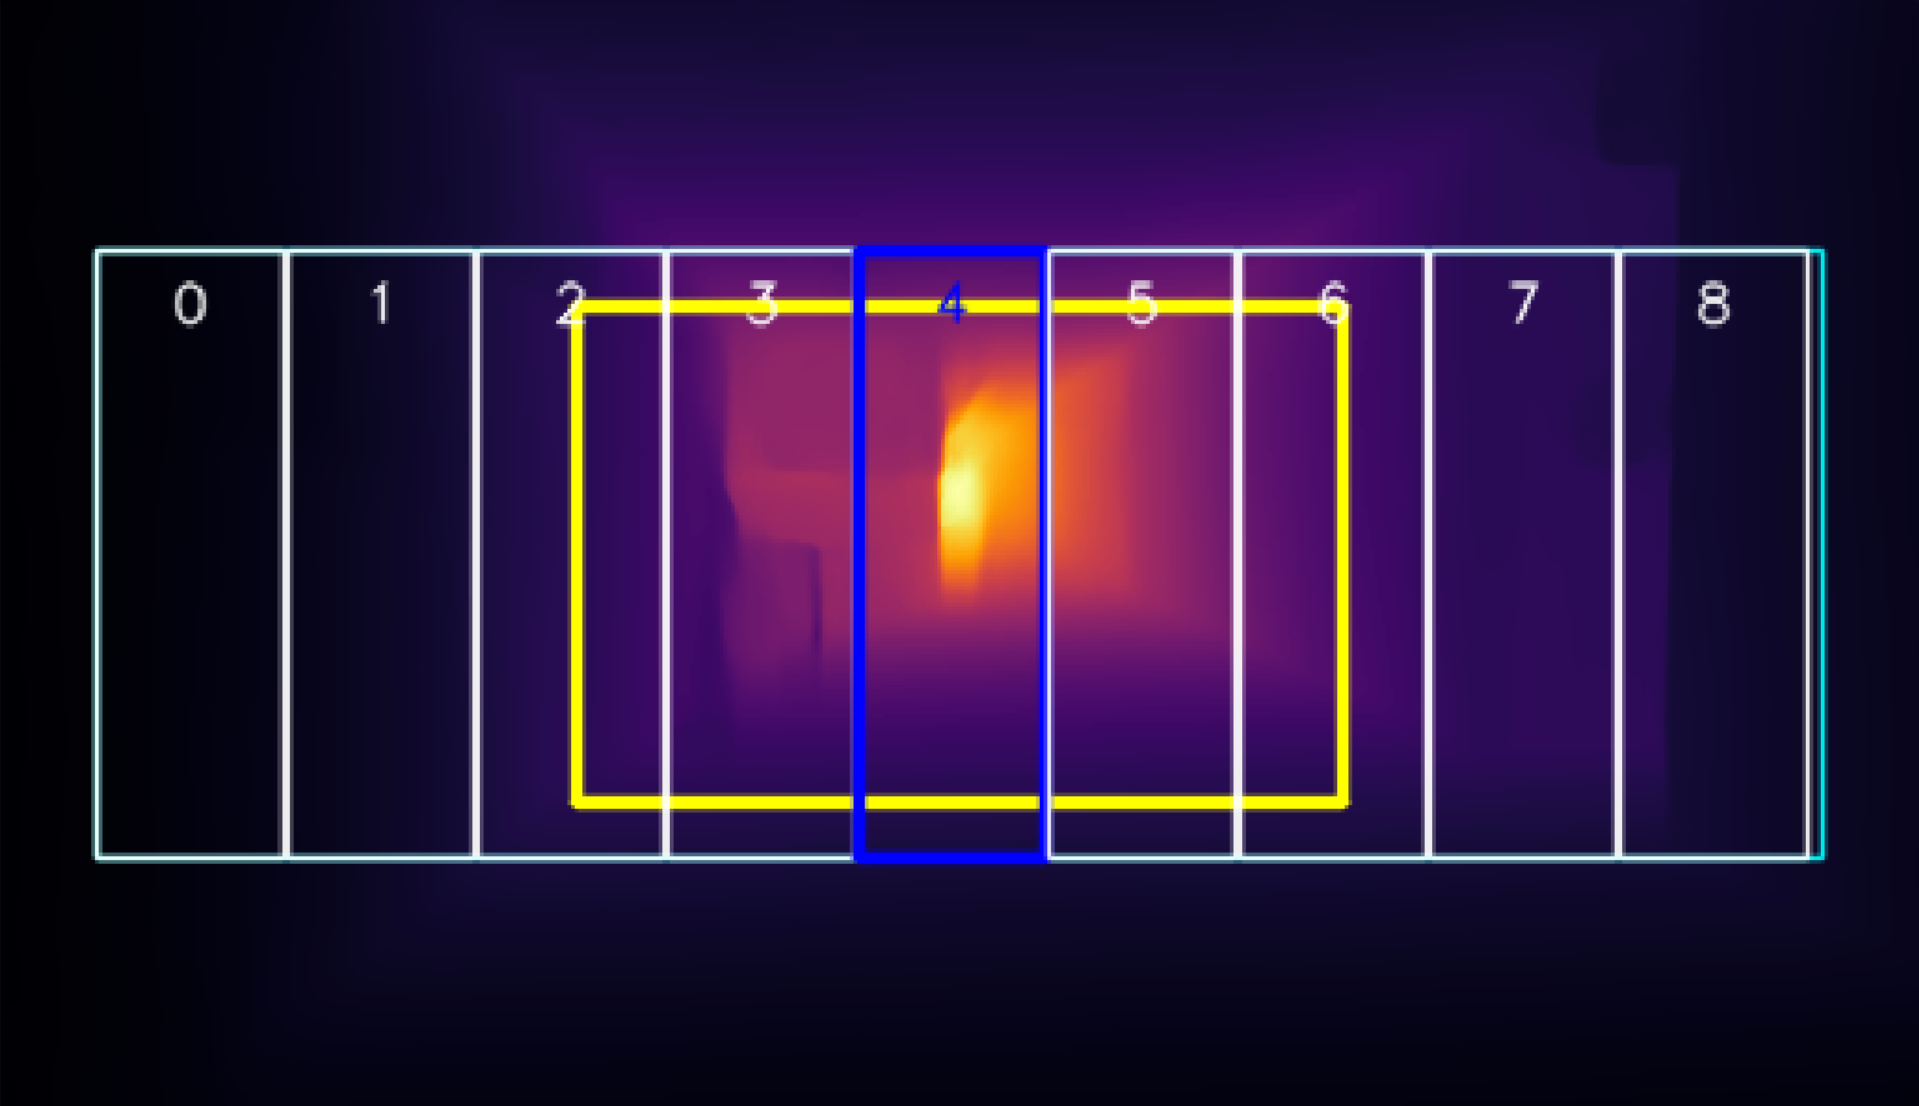
\includegraphics[width=1\textwidth]{images/sectors_ex.png}
    \caption{ROI de guiado dividida en 9 sectores verticales, en azul el sector seleccionado. Fuente: Elaboración propia}
    \label{fig:sectors}
\end{figure}

En cada sector se evalúan dos aspectos principales. En primer lugar, se calcula la profundidad normalizada media, que 
indica si esa zona de la imagen corresponde, en promedio, a una región lejana. Un valor alto indica que el sector 
corresponde, en promedio, a una zona relativamente más despejada dentro de la imagen. En segundo lugar, se calcula la 
proporción de píxeles cercanos, es decir, 
aquellos cuya cercanía supera el umbral definido para detectar ocupación próxima.

A partir de estas dos magnitudes se asigna una puntuación de espacio libre a cada sector:

\[
g_i = \overline{D}_{n,i} - \lambda \rho_i,
\]

donde \(\overline{D}_{n,i}\) es la profundidad normalizada media del sector \(i\), \(\rho_i\) es la proporción de píxeles 
cercanos dentro de dicho sector y \(\lambda\) es un factor de penalización. Esta penalización permite descartar sectores 
que, aunque puedan parecer relativamente profundos en promedio, contienen una cantidad significativa de píxeles cercanos 
y, por tanto, no son adecuados como dirección de evasión.

Una vez calculada la puntuación de todos los sectores, se selecciona aquel que presenta el mayor valor:

\[
i^\star = \arg\max_i g_i.
\]

El sector \(i^\star\) se interpreta como la dirección lateral preferente dentro de la ROI de guiado según la puntuación 
definida. Sin embargo, no se toma simplemente el centro geométrico del sector como punto objetivo, sino que se calcula un 
centroide ponderado hacia las zonas más lejanas. Para ello, cada píxel del sector recibe un peso proporcional a su 
profundidad normalizada, elevando el peso al cuadrado, de manera que los píxeles correspondientes a regiones lejanas 
tengan más influencia en el cálculo del punto objetivo que aquellos situados en zonas menos despejadas.

\[
w(x,y)=D_n(x,y)^2.
\]

El punto objetivo dentro del sector seleccionado se calcula como:

\[
\mathbf{p}^\star =
\frac{\sum w(x,y)\,[x\;\;y]^T}{\sum w(x,y)}.
\]

De esta forma, el punto \(\mathbf{p}^\star\) queda desplazado hacia la zona más libre del mejor sector. Si no existe 
suficiente información válida para calcular este centroide ponderado, se utiliza como alternativa el centro geométrico 
del sector seleccionado.

A continuación, se calcula un vector desde el centro de la imagen hasta el punto objetivo:

\[
\mathbf{u} = \mathbf{p}^\star - \mathbf{p}_c,
\]

donde \(\mathbf{p}_c\) representa el centro de la imagen. Este vector indica hacia qué zona de la imagen debería 
desplazarse el UAV para evitar el obstáculo. En coordenadas de imagen, una componente horizontal positiva indica una 
dirección hacia la derecha, mientras que una componente horizontal negativa indica una dirección hacia la izquierda.

Para evitar cambios bruscos entre fotogramas consecutivos, la dirección obtenida se suaviza temporalmente mediante un filtro 
exponencial:

\[
\tilde{\mathbf{u}}_t =
\alpha_u \tilde{\mathbf{u}}_{t-1} + (1-\alpha_u)\mathbf{u}_t.
\]


Finalmente, se normaliza para obtener el vector final de evitación:

\[
\mathbf{v}_t =
\begin{cases}
\dfrac{\tilde{\mathbf{u}}_t}{\|\tilde{\mathbf{u}}_t\|}, & \text{si } \|\tilde{\mathbf{u}}_t\| > \varepsilon,\\[2mm]
\mathbf{0}, & \text{en otro caso,}
\end{cases}
\]

donde \(\varepsilon\) es un umbral pequeño positivo que evita la división por valores cercanos a cero cuando la dirección de evasión no queda suficientemente definida.

Por tanto, el vector \(\mathbf{v}_t\) representa la dirección normalizada hacia la zona más segura de la imagen, y posteriormente se convierte en un ángulo de evasión 
para devolverlo como \textit{evade\_angle}, Figura~\ref{fig:evade_angle}.

\[\textit{evade\_angle} = \mathrm{atan2}(v_y, v_x).\]



\begin{figure}[H]
    \centering
    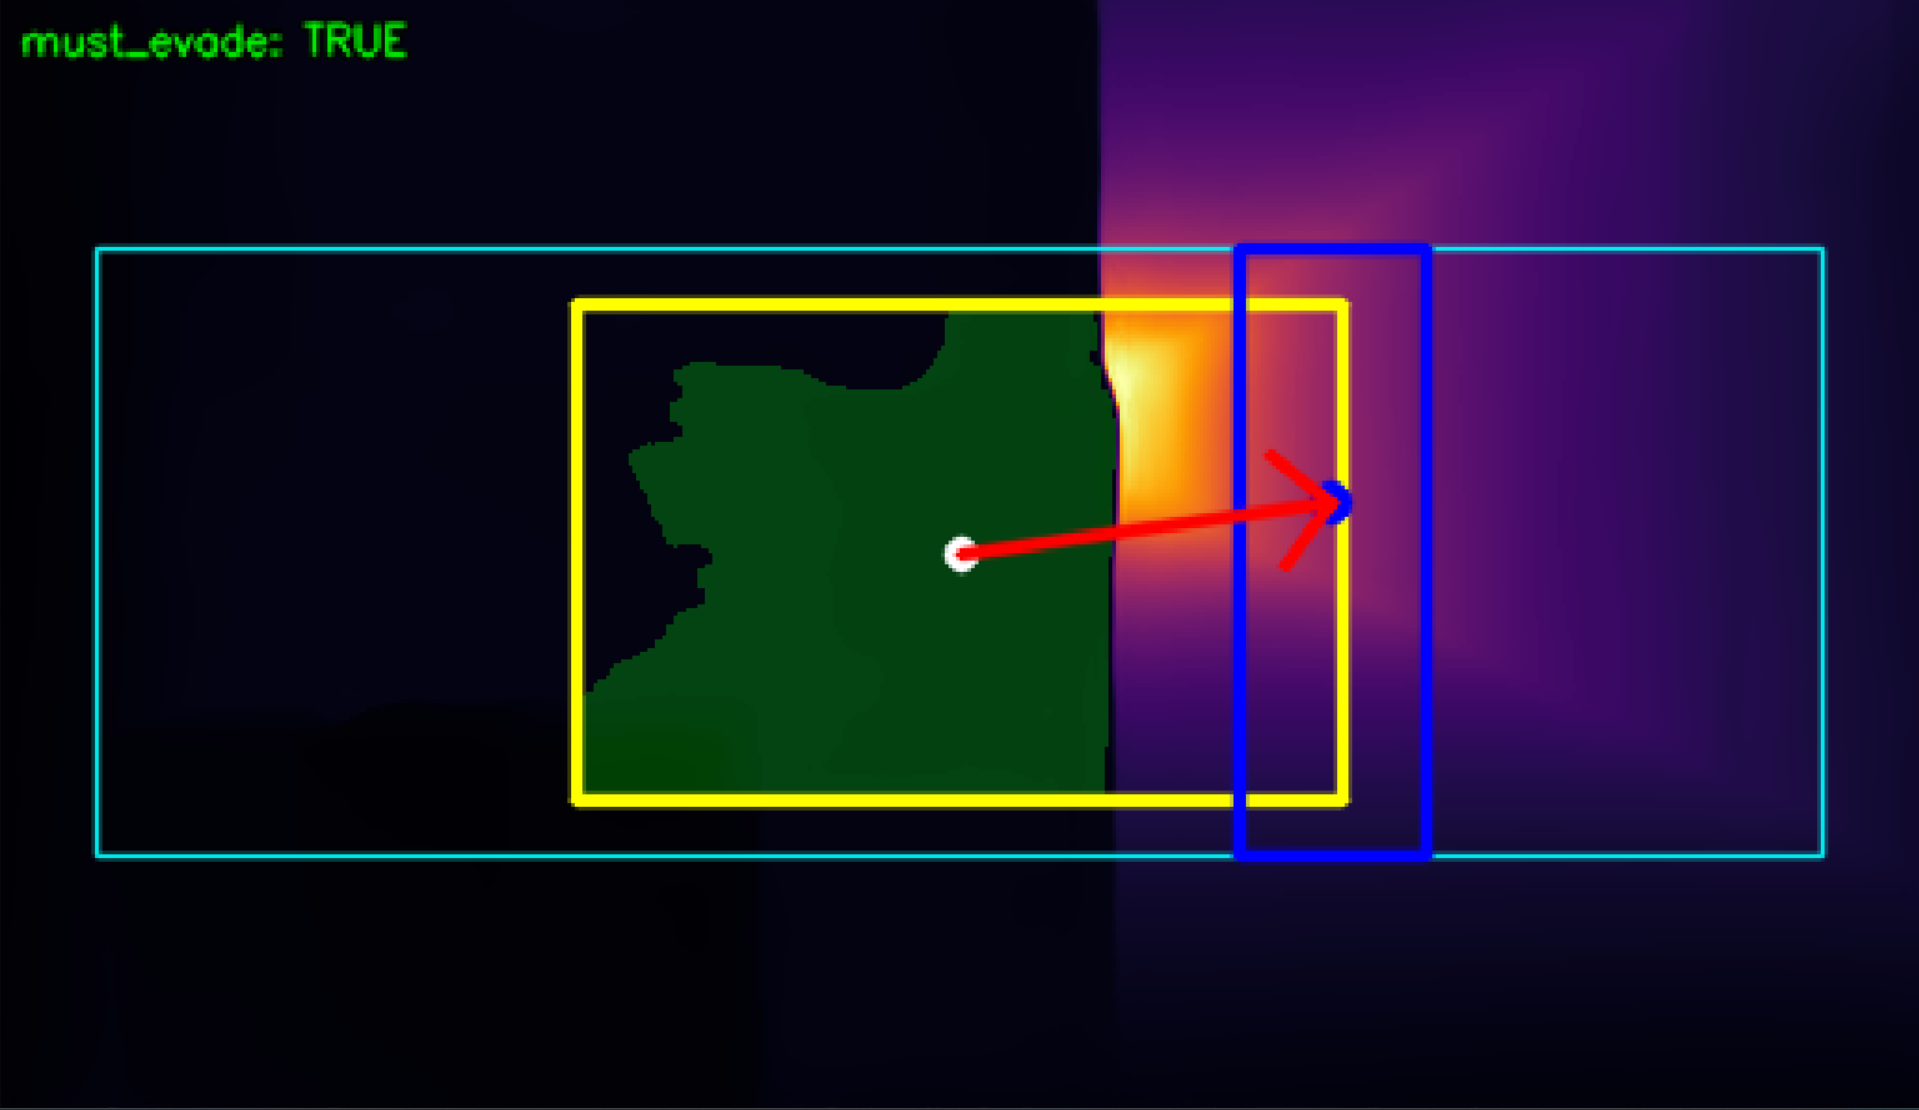
\includegraphics[width=1\textwidth]{images/evade_angle.png}
    \caption{La flecha indica la dirección de evitación decidida por el algoritmo. Fuente: Elaboración propia}
    \label{fig:evade_angle}
\end{figure}

\subsection{Interpretación}

La filosofía del algoritmo es desacoplar dos problemas distintos:

\begin{itemize}
\item \textbf{detección}: decidir si existe un obstáculo frontal suficientemente relevante como para activar evasión;
\item \textbf{guiado}: decidir hacia qué dirección conviene desplazarse una vez detectado el obstáculo.
\end{itemize}

La detección se apoya en indicadores de ocupación y cercanía frontal, mientras que la dirección se basa en la selección 
del sector con mejor puntuación de guiado. Esta separación hace al sistema más robusto que una aproximación basada 
únicamente en el gradiente medio del mapa de profundidad como se realizó en primera instancia en el proyecto de 
investigación tutelado~\cite{estudio-nav2D}.

El planificador, por tanto, recibirá las tres variables (\textit{must\_evade}, \textit{evade\_angle} y 
\textit{obstacle\_score}). En el momento en que la bandera de activación se ponga a 1, el algoritmo de planificación 
local empezará a tener en cuenta el ángulo de evitación o escape, y podrá decidir también la intensidad que debe aplicar 
a esta acción mediante la puntuación. En las siguientes gráficas de las Figuras~\ref{fig:avoidance_angle},~\ref{fig:avoidance_mag} y \ref{fig:avoidance_flag} se puede observar 
la salida de estas tres variables para un recorrido con dos obstáculos (la tercera activación de la bandera booleana corresponde al aterrizaje del dron).

\begin{figure}[H]
    \centering
    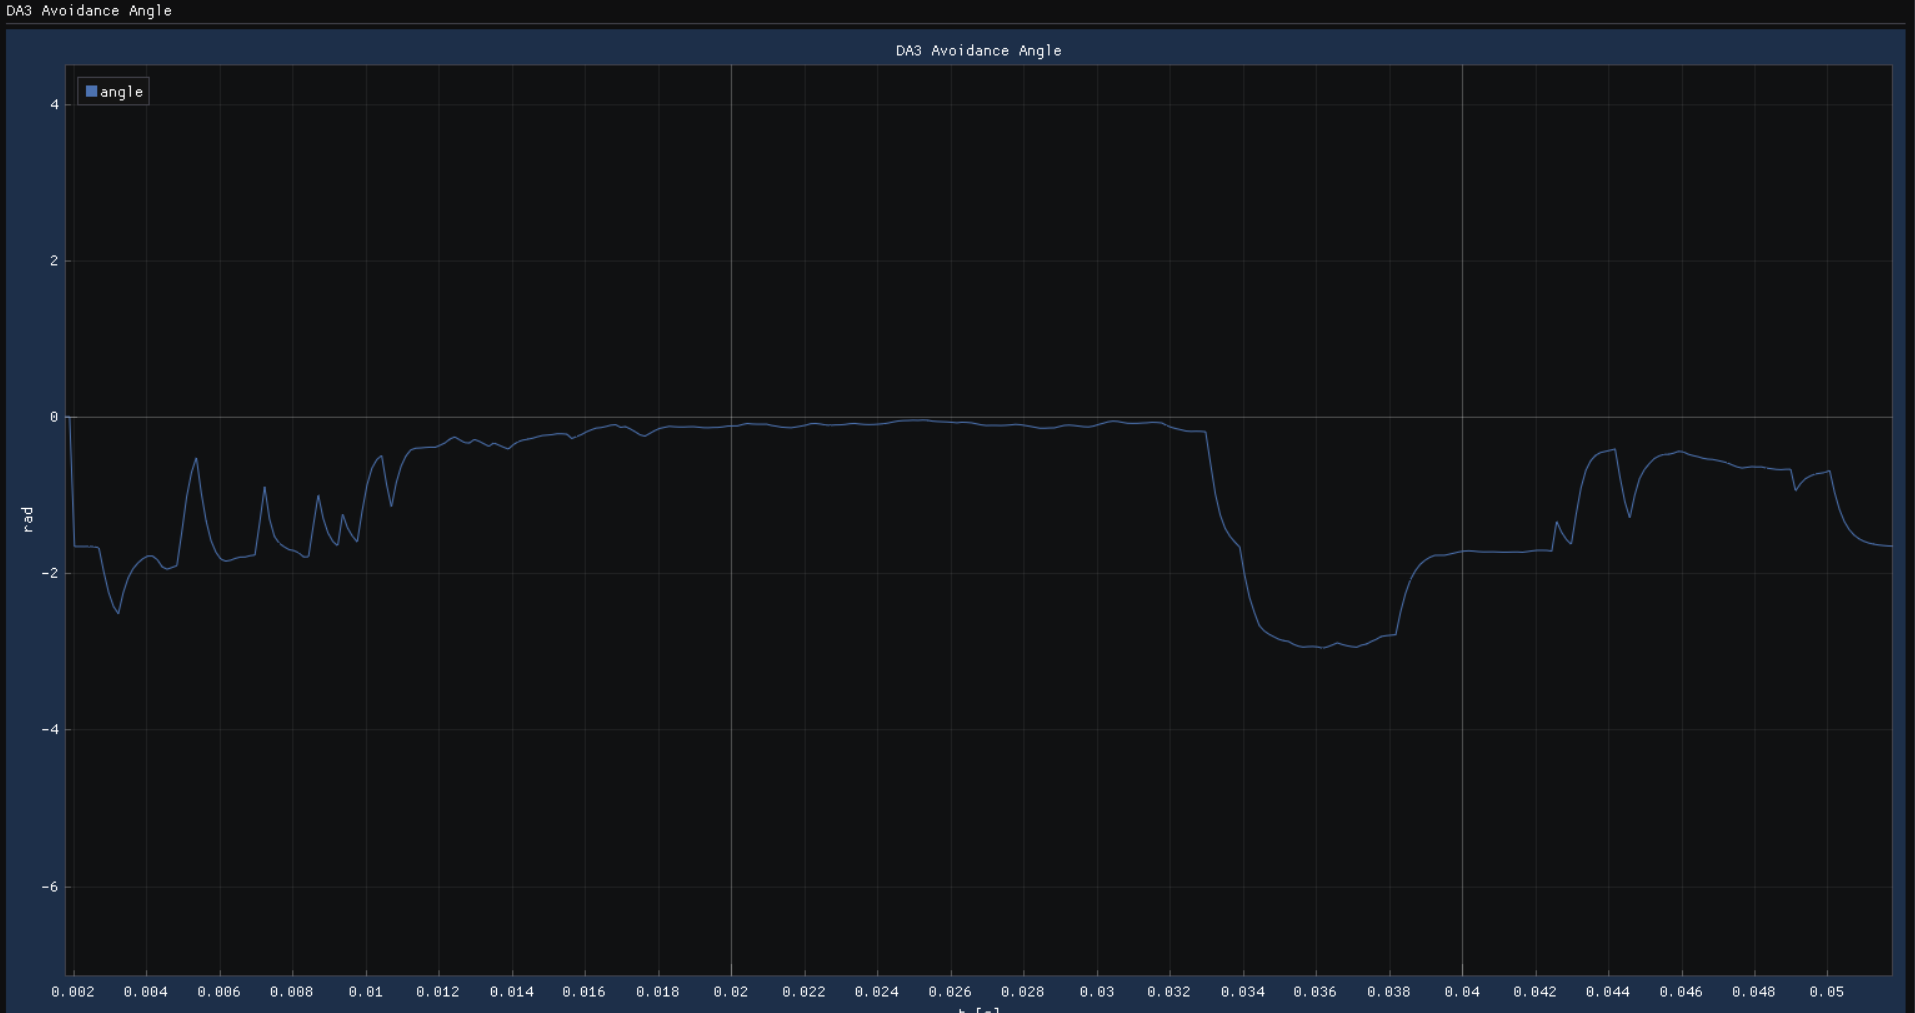
\includegraphics[width=1\textwidth]{images/avoidance_angle.png}
    \caption{Ángulo de evitación. Fuente: Elaboración propia}
    \label{fig:avoidance_angle}
\end{figure}

\begin{figure}[H]
    \centering
    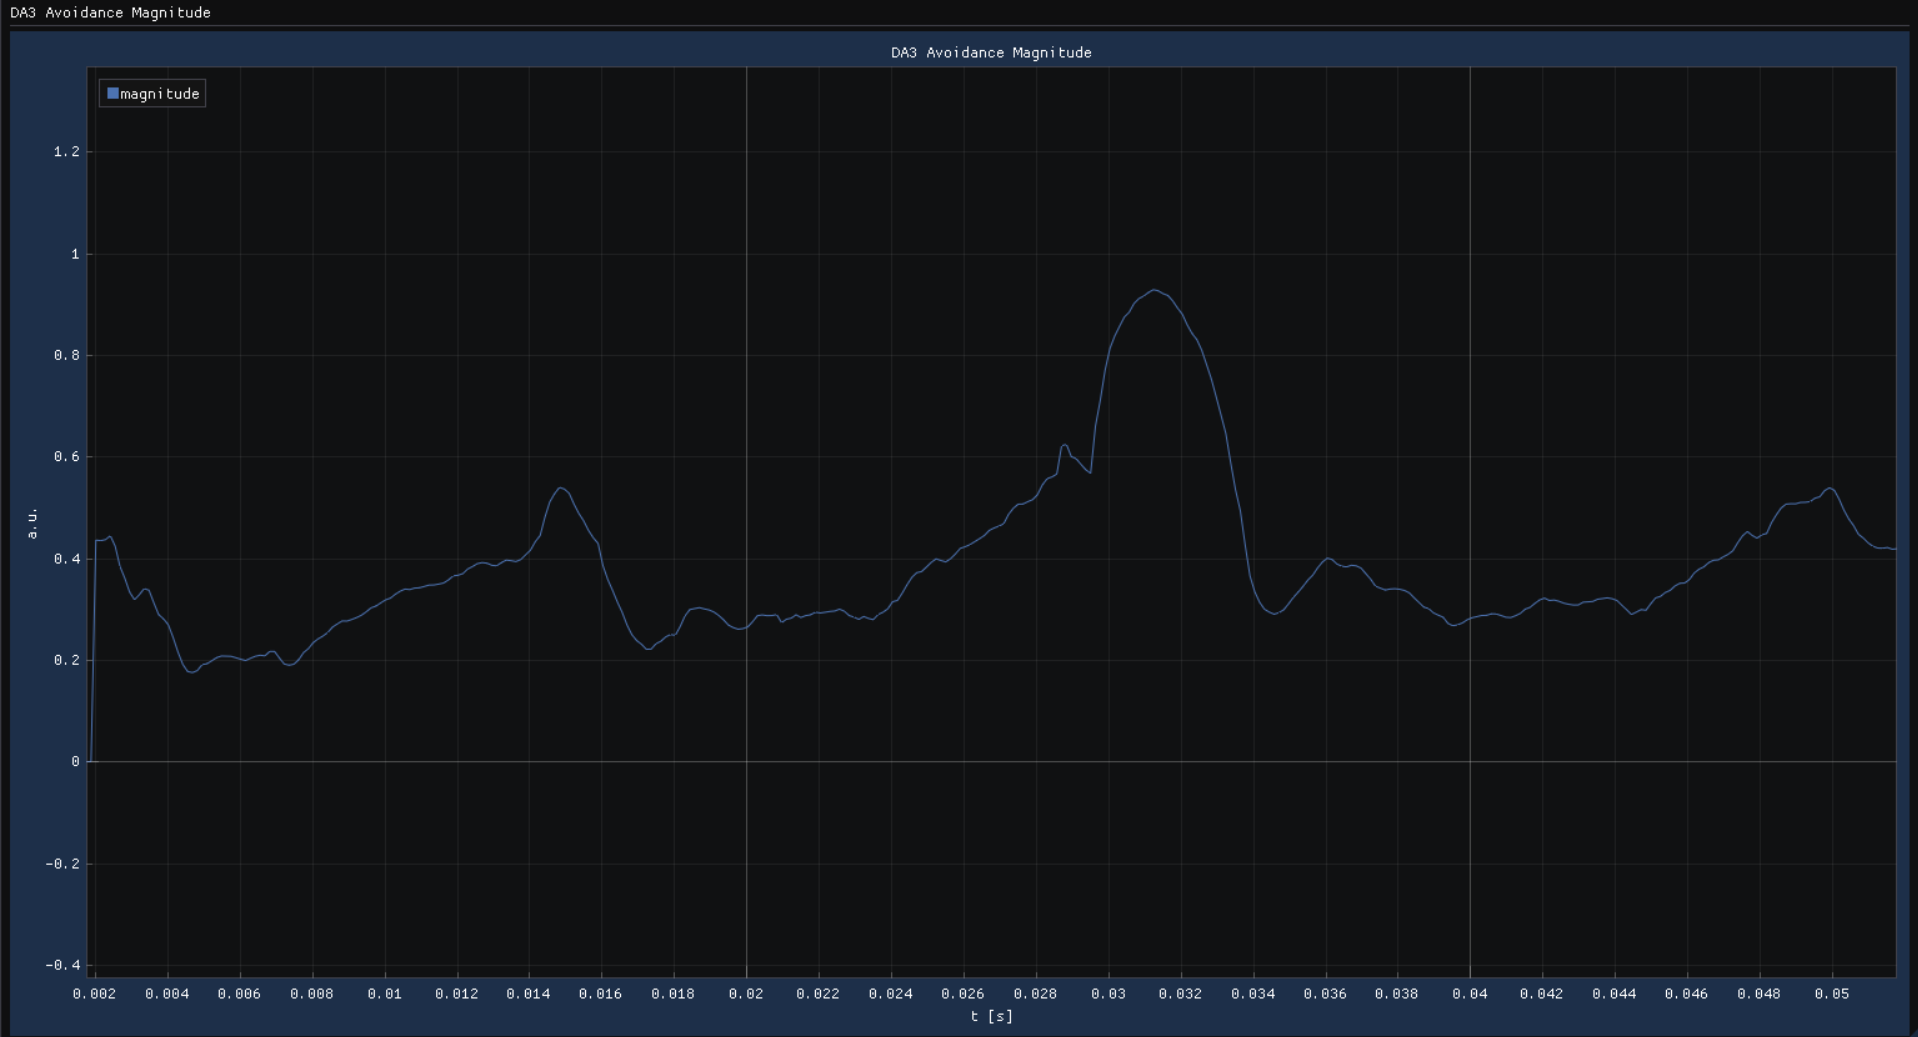
\includegraphics[width=1\textwidth]{images/avoidance_mag.png}
    \caption{Puntuación de obstáculo. Fuente: Elaboración propia}
    \label{fig:avoidance_mag}
\end{figure}
\begin{figure}[H]
    \centering
    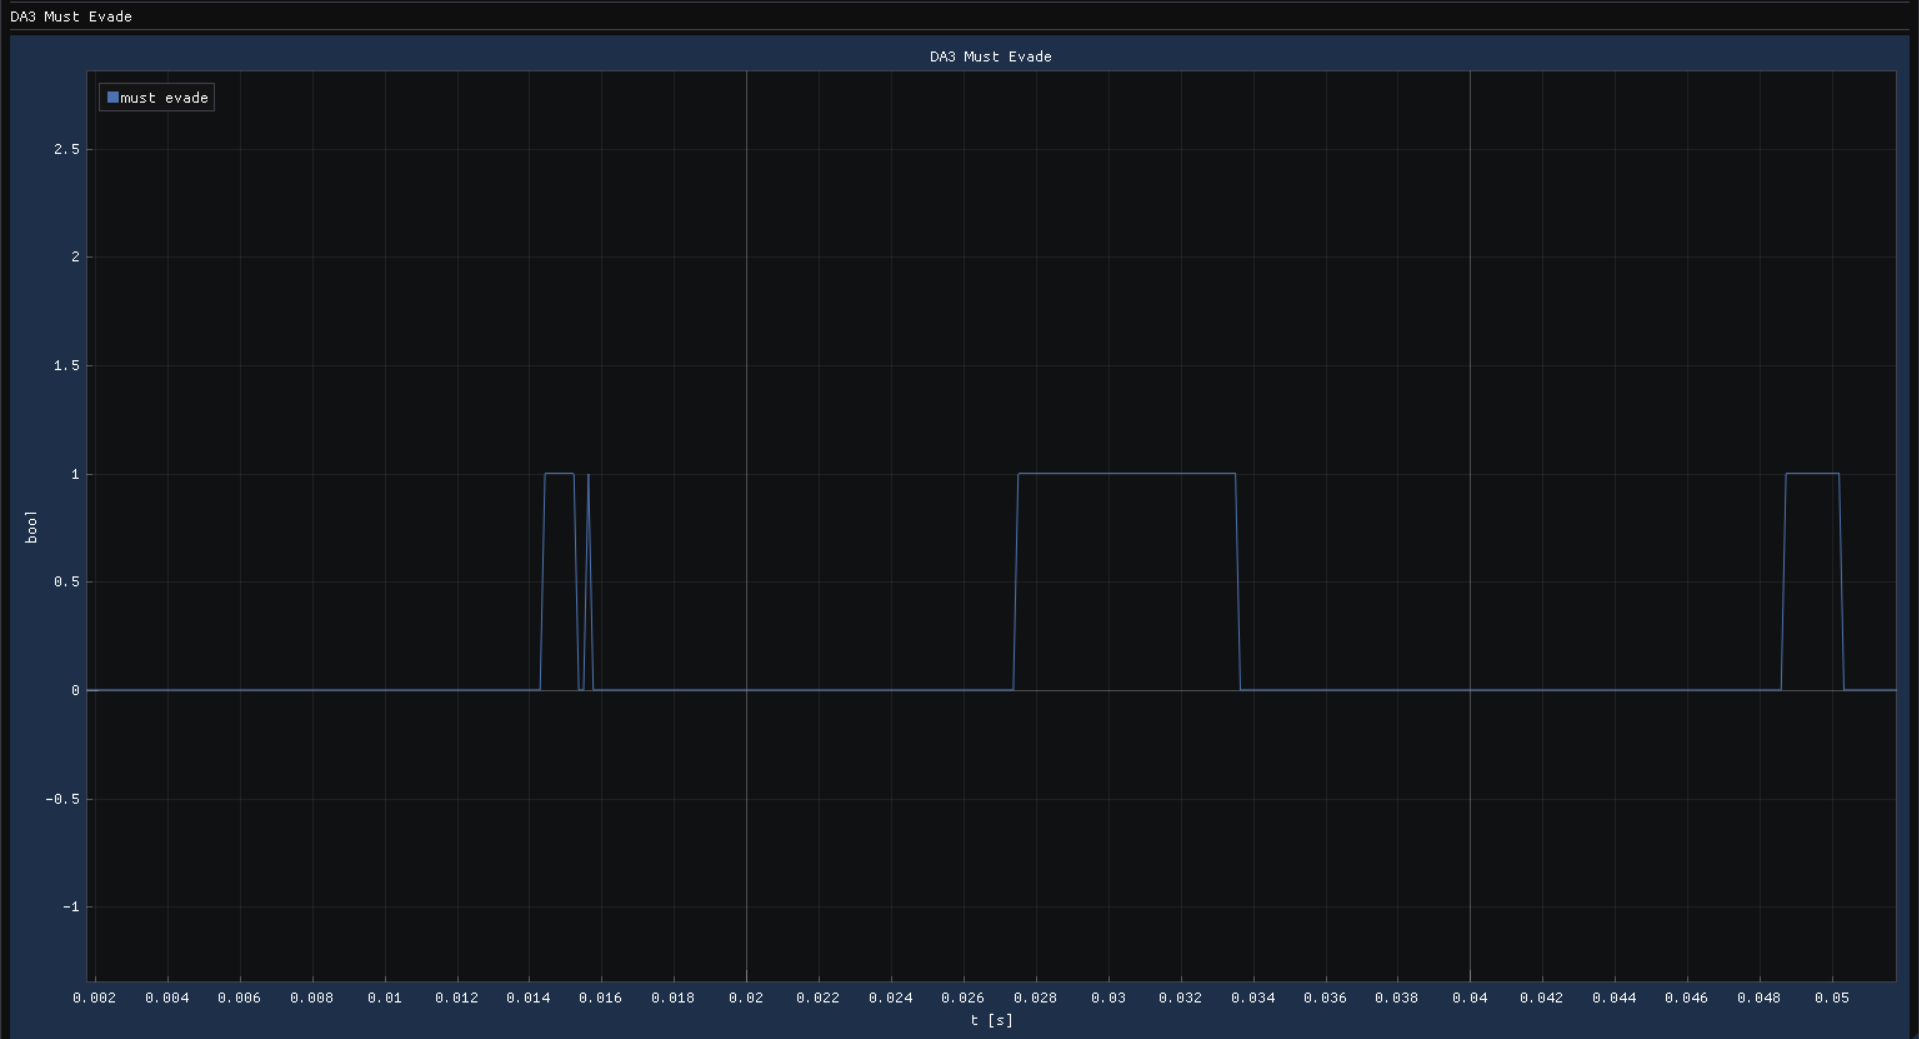
\includegraphics[width=1\textwidth]{images/avoidance_flag.png}
    \caption{Bandera de evitación booleana (1 activada, 0 desactivada). Fuente: Elaboración propia}
    \label{fig:avoidance_flag}
\end{figure}
